\section{x86}

\begin{itemize}
    \item Assembler produces \textit{object} that contains \textit{segments} (address ranges with a purpose)
    \item Segments (labels) containing runnable code: \texttt{.text}
    \item Segments containing initialised data: \texttt{.data}
    \item Remember to specify segment to fit purpose:
    \item Specifying data: \texttt{.ascii} and \texttt{.asciz}
    \item Metadata: \texttt{.func}, \texttt{.type}, \texttt{endfunc}, \texttt{.size}, \texttt{.globl}
\end{itemize}

\begin{figure}[h]
    \centering
    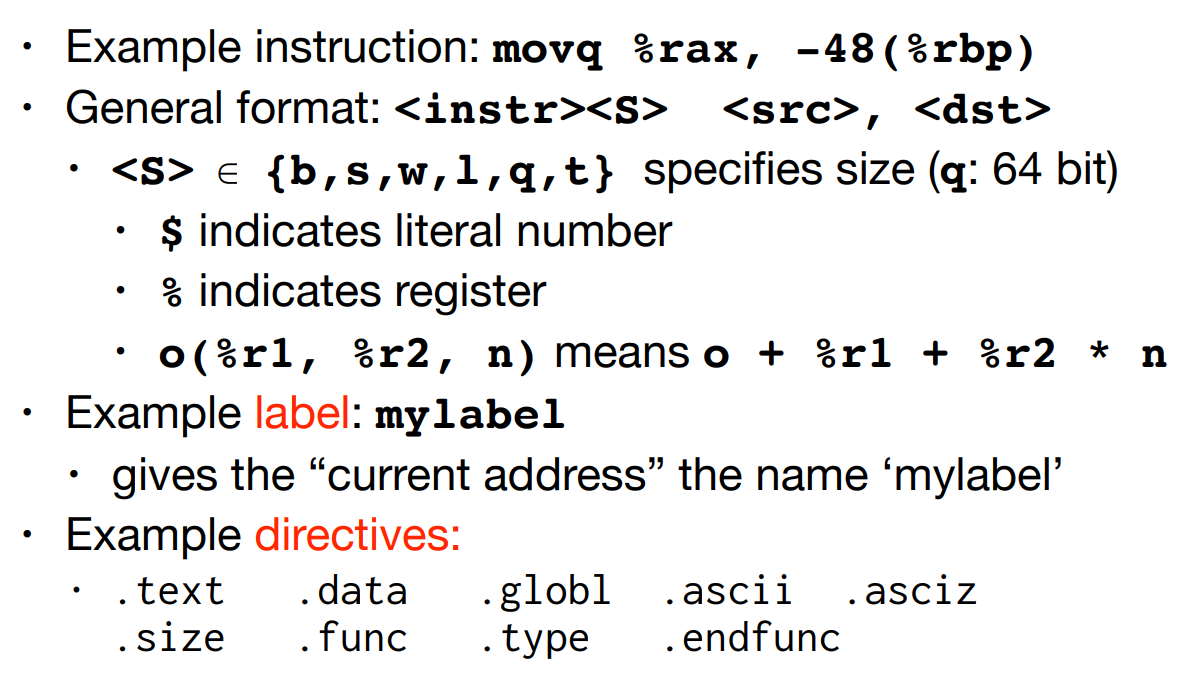
\includegraphics[scale=0.3]{assets/x86.PNG}
    \caption{X86 language}
    \label{fig:x86}
\end{figure}

\subsection{Stack}

Active functions are placed on top of eachother on the stack. Allocate the maximum amount of memory that each function needs for its locals, temps, etc.\\

This can be statically analysed, as we can count the amount of variables and time this with the biggest size of a single variable.\\

\texttt{SP} is the stack pointer (the top), while \texttt{FP} is a pointer to the top of the last function call stack. See figure \ref{fig:stack}.

\begin{figure}[H]
    \centering
    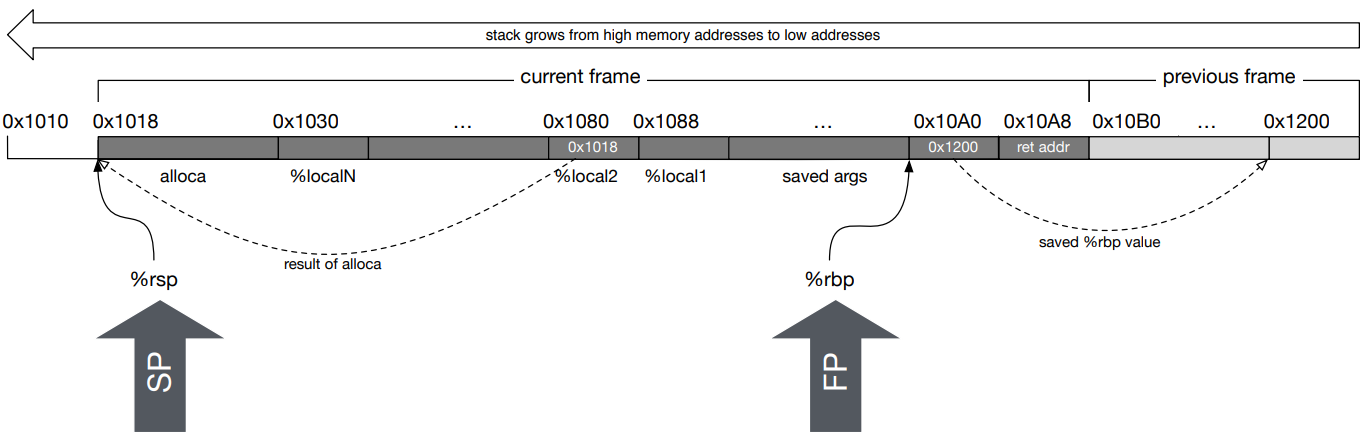
\includegraphics[width=\textwidth]{assets/stack.PNG}
    \caption{Stack growth (\texttt{SP}, and \texttt{FP})}
    \label{fig:stack}
\end{figure}

\subsection{Registers}
RBP, RBX, and R12-R15 are callee save registers, i.e. preserved across functions. \textbf{Don't use}.\\

\textbf{System V x86 ABI}: Application Binary Interface. Document describing frame organization, calling conventions and register purposes. See figure \ref{fig:sys_abi}.\\

4-6 parameters can be saved on register, the rest should be stored in the stack. This is because loading values from registers is much faster, so if possible, use only registers.

\begin{figure}[H]
    \centering
    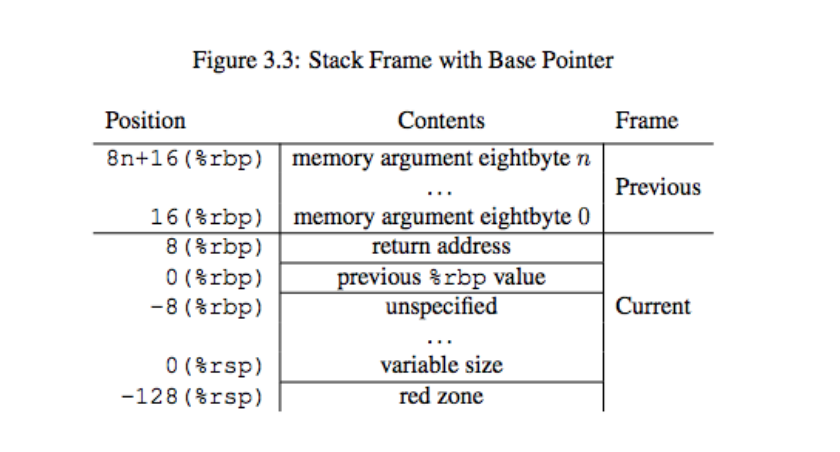
\includegraphics[scale=0.5]{assets/system V ABI.PNG}
    \caption{System V ABI stack frame and Base pointer}
    \label{fig:sys_abi}
\end{figure}

\newpage

\section{Liveness Analysis}
To save resources some registers can be merged. Liveness analysis shows which are safe to merge.\\

\begin{itemize}
    \item Variable is live at a point in and execution if its value is needed in the future.
    \item \textbf{Static liveness}: The value is definitely not needed vs. may be need in the future.
    \item \textbf{Interference graph}: See figure \ref{fig:interference}. Variables are live if their value is used in a future execution execution. For example the value $c$ is live on all transitions. The value $a$ is live on transitions \{$1\rightarrow 2$, $4\rightarrow 5$, $5\rightarrow 2$\}.
    \begin{itemize}
        \item Interference exists among to variables $v,w$ if they have overlapping liveness path (Are alive during same transition).
        \item \texttt{MOVE} instruction moves same value into another register, therefore, these two registers can be merged even if they have interference.
    \end{itemize}
\end{itemize}

\begin{figure}[H]
    \centering
    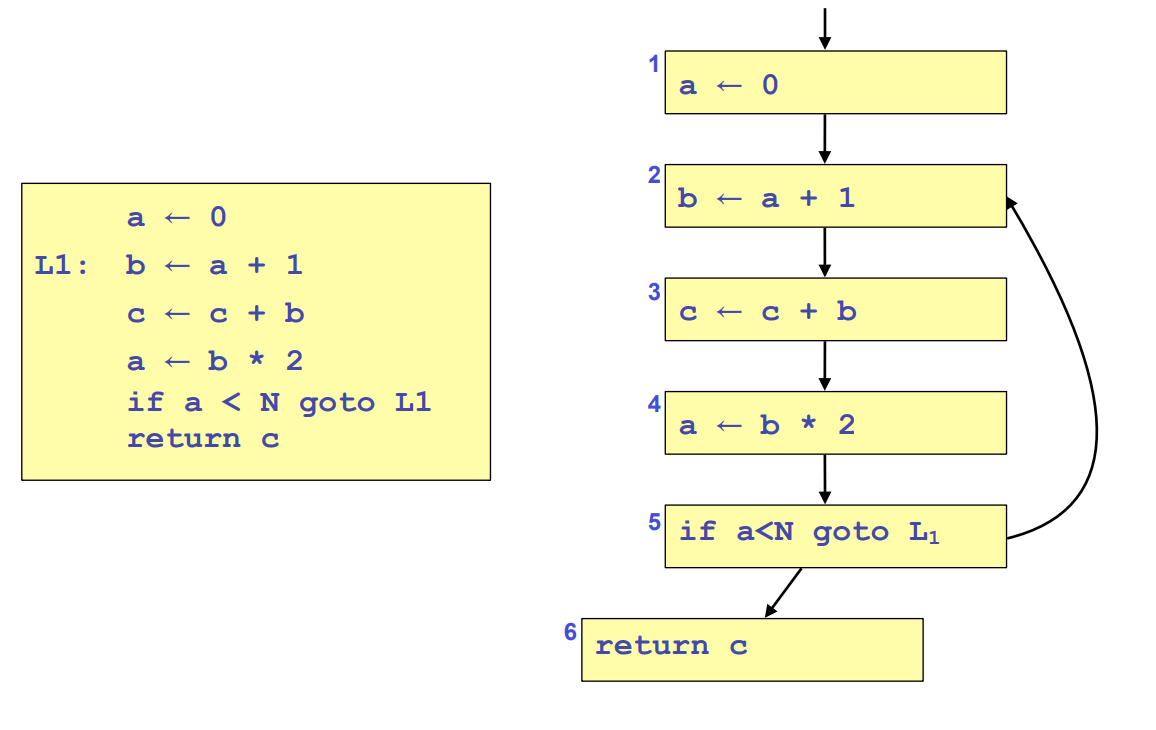
\includegraphics[scale = 0.35]{assets/interference graph.PNG}
    \caption{Interference graph example}
    \label{fig:interference}
\end{figure}

\begin{figure}[H]
    \centering
    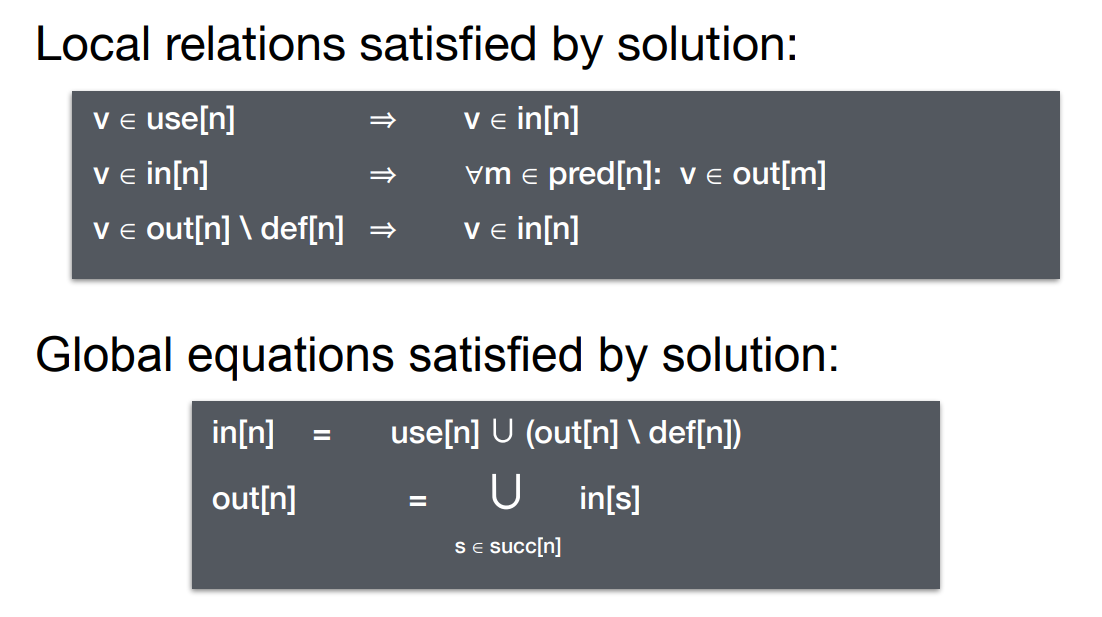
\includegraphics[scale = 0.5]{assets/liveness.PNG}
    \caption{Liveness}
    \label{fig:liveness}
\end{figure}

\begin{figure}[H]
    \centering
    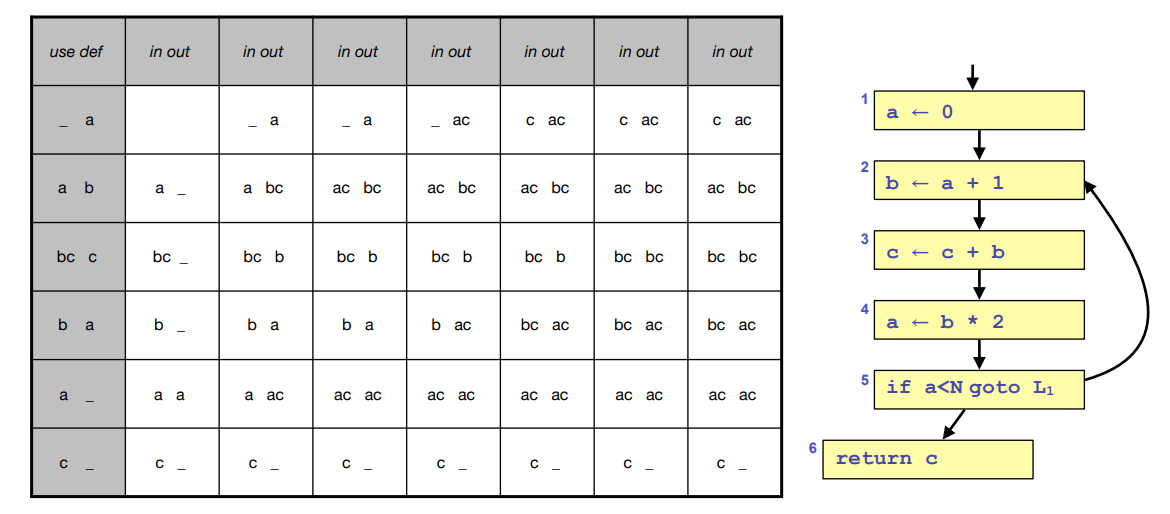
\includegraphics[scale = 0.55]{assets/liveness_example.PNG}
    \caption{Liveness Example}
    \label{fig:liveness}
\end{figure}
